\documentclass{article}
\usepackage[a4paper, tmargin=1in, bmargin=1in]{geometry}
\usepackage[utf8]{inputenc}
\usepackage{graphicx}
\usepackage{parskip}
\usepackage{pdflscape}
\usepackage{listings}
%\usepackage{hyperref}
%\usepackage{titlesec}

\newcommand{\ra}{$\rightarrow$}


\title{EE 344 Project Proposal \\ Visible Light Communication using LED}
\author{
  Arka Sadhu - 140070011\\
  Sudeep Salgia - 14D070011\\
  Parth Kothari - 14D070019\\
}
\date{January 2017}

\begin{document}
%\maketitle

% \tableofcontents
% \newpage
\section{Work Accomplished }
% Five to ten sentences providing a non-technical description; use technical words only to describe important specifications. Describe the “big picture” of the project.

\subsection{Reading Literature}

During the first week, each of us went through a number of papers in the field of visible light communication and brainstorming simulataneously. The papers included a wide variety of theoretical aspects regarding the basic concept, however did not extensively cover about the implementation issues. 

\subsection{Software Implementation}

\subsection{Hardware Implementation}

Transmitter circuit: The current circuit comprises an inverter which drives the LED according to the input signal. The waveform input to the LED follows the bit stream upto 1Mhz. The LED is biased using a pull up resistor to make the ensure a certain level of brightness of the LED while transmitting. \\

Receiver Circuit: It consists of a photodetector (BPW34), followed by an amplifier and a high pass filter to remove the 50hc noise due to ambient light. We have currently tested number of designs for the filter by simulating them on LT spice. We are still working on the exact specifications of the filter taking into consideration a number of factors.%like the slew rate of the opamps, its capacitive effects, power required for rail voltages in the final circuit. 


\section{Testing}

We tested each of the components in a sequential manner in order to ensure the integrity of each component.
\begin{itemize}
\item The voltage waveform at the output of the LED driving circuit. It was ensured it followed the input. 
\item The voltage waveform at the output of the amplifier was tested using a DSO and was resembling the input waveforms reasonably well upto $75$ khz. 
\item The distance between the LED and the photodetector was gradually increased upto 50 cm and we could receive the transmitted waveform accurately upto $40$ khz. 
\item Finally, we gave the input(a single character) from our laptop through the USB to UART converter and received it through another USB to UART converter on another laptop. We successfully the reception for a range of angles and a distances upto 10 cm and for frequencies upto 40khz. 
\item We have tested the receiver circuit separately and it had a good response upto $200$kHz before distorting. We are thus looking for better designs.
\end{itemize}

\section{Problems Faced}

\begin{itemize}
% ******************************************** 
% ARKA FILL SOFTWARE KE PAINS HERE
%
%***************************************




\item{We initally had tried to drive the LED using MOSFET IRF$840$ but there seemed to an issue which we couldn't quite figure out the reason for and hence tried the inverter which gave good results.}
\item{Another issue was with the choice of OPAmp. We had begun with using ua741 which had a very poor slew rate and hence distorted the waveforms. We switched to TL$082$ which has a slew rate sufficient for our application.}
\item{ Another issue is about the design of the filter. We tried we a simple first order high pass filter which gave poor results even at frequencies as low as $20$kHz due to capacitive effects. We resorted to a higher order filter which gave better results. Currenty, the issue is about to understand the real bottleneck among the Opamp, the filter design and or capacitive effects of the breadboard at these frequencies.}

\end{itemize}

\section{Work Promised}

\begin{itemize}
\item Understanding the literature
\item Procurement of components : The SD card reader is yet to arrive. We have placed an order for the same.
\item Finishing the transmitter ciruit
\item Getting started with the receiver circuit
\end{itemize}

\section{Goals for the next evaluation}

\begin{itemize}
\item Transmit files asynchronously upto data rates of $100$kbps successfully
\item Integrate the circuits and add a PLL for synchronous reception and ensure reception of a basic toggling waveform
\item Code the modulation the demodulation schemes in the microcontroller
\end{itemize}





% summarize what your design project is to achieve. It can be   general and non-technical but should describe “the big picture” elaborately. Basically, you briefly explain what the solution is and what is unique about your solution.

% Our project aims to achieve the the following objectives in order to make a satisfactory prototype
% \begin{itemize}
% \item Transmission speed should be 1 Mb/s
% \item Blinking should not be detected by the naked eye
% \item Link should work over a distance of 50 cm
% \item Should transmit a file stored in a USB/SD card 
% \end{itemize}

% \subsection{Project Specifications}
% \begin{itemize}
% \item Customer Specifications: The following specifications will guarantee a finished product for consumer use
%   \begin{itemize
%   \item Efficient, reliable and accurate transmission of the data at desired high speeds.
%   \item Availability of ambient light, along with the simultaneous data transmission from the LEDs. Also, care will be taken that the flickering of the LEDs would be indiscernible, without compromising much on the illumination.  
%   \end{itemize}
% \item Technical Specifications: 
%   \begin{itemize}
%   \item Data Rate : The speed with which data can be transmitted from one device to another. (Transmitter to Receiver in this case). Our initial aim is to achieve a data rate of 1 Kbps and then increase and finally reach the desired speed of 1 Mbps.
%   \item Bit Error Rate : It is the number of bit errors is the number of received bits of a data stream over a communication channel that have been altered due to noise, interference, distortion or bit synchronization errors. It is given by the formula, in On-Off Keying Modulation Scheme, as $$\textrm{OOK} : \textrm{BER} = \mathcal{N}(\sqrt{\textrm{SNR}})$$ We hope to achieve a BER of $10^{-4}$ and reduce it further if possible.
%   \item Distance : We hope to achieve accurate data transmission upto a distance of 50 cm. If       we are done with the above objectives, we hope to increase the distance till 100 cm.  
%   \end{itemize}
% \end{itemize}

% \section{Technical Design Description}
% \subsection{Possible Solutions and Design Alternatives}
% % In this section describe the possible solutions and evaluate them in terms their possible performance, availability of the resources, and other limitations. State the solution you would like to adopt with justification.
% When it comes to design, there a lot of choices regarding the LED specifications and modulation techniques. There are small tradeoffs with choices of one over another in terms of speed, illumination in the room, power consumption, range of the link etc. The choice depends on the place of deployment and the kind of data we need to transmit. Hence our design parameters can be changed and tweaked keeping mind the following issues. Our aim, however, will be to build a simple demonstrable prototype of a VLC, without delving into the nuances of the parameters\\ 

% There are a number of issues when it comes to implementing VLC with the lights in the room which are to be used for illumination purposes. One of them being that due to modulation and constant variation in intensity to transmit information. This leads to a reduction in the average DC value of the light and hence in the illumination of the roo. Thus it is often task to maintain a basic level of illumination in the room that does not affect anything else. For this the main idea is to increase the frequency of the ones in the encoding scheme so that the average DC value increases. This is done using very simple coding techniques like giving a preference to 1 over 0 in Huffman encoding, etc. However we aim to tackle this problem and work on it and incorporate it into the plan of action once we have finished doing more fundamental aspects like synchronization and clock offset correction.

% \subsection{System-level overview}
% % Include a block diagram with functional description. A brief overview of what   your proposed device/solution is and how it will work. Include figures to illustrate the concept of your final product showing what it will look like, showing how it will work, and showing what it will do.
% \begin{itemize}
% \item WHAT WILL IT LOOK LIKE:\\
%   The final product will essentially consists of 2 components:
%   \begin{itemize}
%   \item The Transmitter: This will consist of a microcontroller (TIVA Board) which will get the data from the USB/SD, encode the data and finally modulate it. The data will then be sent to the LED circuit, driven by the microcontroller, for transmission. The LED circuit as mentioned earlier will essentially be used to drive the LED and ensure proper biasing. If time permits, we wish to make the LED circuitry on a PCB. Thus, the transmitter side consists of a microcontroller and LED circuit.
%   \item The Receiver : The transmitted signal will be received by the Receiver circuitry. This circuitry will consist of an amplifier to amplify the received signal which will then be sent to the microcontroller. The phase offset and clock synchronisation will either be done by PLL or by the microcontroller. We will try both alternatives and choose whichever works better. After synchronisation, the microcontroller will demodulate the signal and finally decode it to get the original message. Again, if time permits, we will make a PCB of the receiver circuit also.
%   \end{itemize}
% \item HOW IT WILL WORK:\\
%   The following is the step-by-step description of the entire system right from acquisition of the data to its reception in a file on the computer.
%   \begin{itemize}
%   \item Data Input - The data will be first acquired by the microcontroller from the SD card. 
%     % \item Encoding - The Input Data will then be encoded using Hoffman Encoding (CHECK) to reduce the number of bits to transmit
%   \item Modulation - The encoded data will then be modulated and thus converted to a form which can be transmitted through the optical Channel via the LEDs (the Transmitter).
%   \item Channel - In visible light communication, it is pretty obvious that the data will be transmitted through an optical channel. Errors may arise due to interferences amongst symbols, or addition of noise or multipath fading
%   \item Frequency Offset Correction and Clock Synchronisation at the Receiver- The receiver will be more complicated in design than the transmitter because of this feature. Appropriate circuitry will be designed to correct the frequency offset and synchronise the clocks
%   \item Demodulation - Once the point mentioned above, gets implemented correctly, the modulated data will be demodulated to recover the encoded data
%   \item Decoding - The encoded data will be decoded to retrieve the original data intended to be sent
%   \item Saving the data - Finally the data which is received will then be saved in a file on the computer
%   \end{itemize}
% \item WHAT IT WILL DO:\\
%   The project on completion will be capable of accomplishing the following tasks:
%   \begin{itemize}
%   \item Efficient, reliable and accurate transmission of the data at a speed of 1 Mbps.
%   \item Transmission of a file stored in a USB or a SD card
%   \item Accurate transmissions upto a distance of 50 cm
%   \item Provision for ambient lighting for aesthetic effects along with transmission.  
%   \end{itemize}
% \item Functional Diagram:\\
%   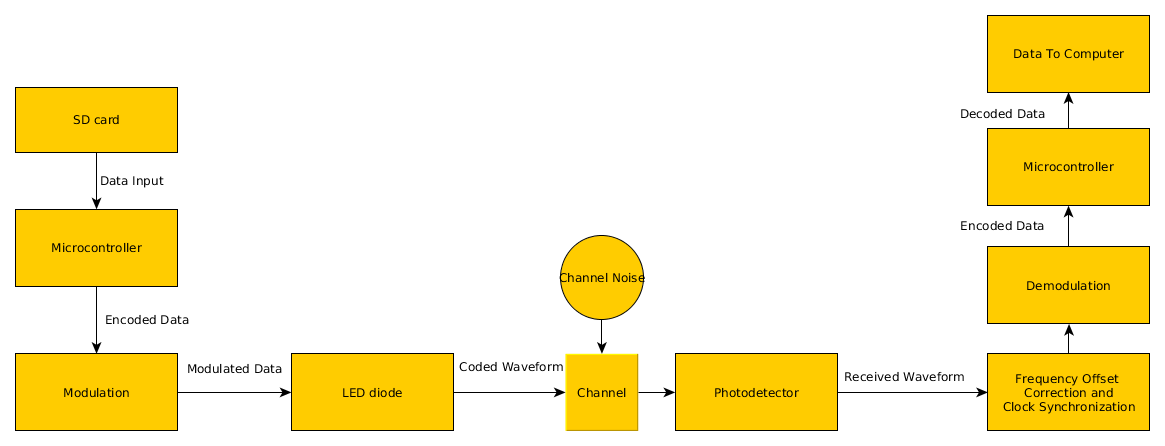
\includegraphics[scale=0.4]{functional_flow}
  
% \end{itemize}


% \subsection{Performance Validation}
% % Describe how you would validate your final design and prove that it meets the specifications you promised. You would demonstrate your successful project at the final Design Lab Demo.
% The following measures will be noted will be used to values our performance by keeping a distance of 50 cm between the LED and the receiver:
% \begin{itemize}
% \item Time required to transmit given data from the LED to the receiver and thus the Data Rate
% \item The Bit Error Rate (BER) - By comparing the input file with the received file
% \end{itemize}

% \section{Project Plan}
% % This section is to provide 
% % A listing of all tasks, planning, involving all the tasks and sub-tasks. A task can be defined as anything that takes your time.
% % Examples of tasks possible are (but not limited to):  Embedded system design, sensor testing, analog module design and testing, mechanical design, PCB    design, power consumption estimation, components procurement, documentation, etc.

% Tasks to be done:
% \begin{itemize}
% \item Reading Literature :  We would need to go through a basic survey regarding the basics of visible light communication, corresponding hardware, modulation techniques with pros and cons of each of them, and hence come with a viable solution incorporating the all the factors and the feasibility given the availability of components and time constraints. The sources mainly comprise a number of papers and the few books in the field
% \item Circuit design :  Broadly speaking there would be two main parts to this, the transmitting circuit and the reception circuit. The transmission circuit would mainly involve the LED, a biasing circuit, and a switching circuit to generate the bit pattern amongst other basic elements. The reception circuit, which is relatively more difficult would mainly involve a photodetector,a circuit to nullify the ambient DC value and related basic elements.
% \item Generation of bit stream :  Another task is about taking a file and converting it into a bit stream which can be used to drive or feed the switching circuit. The main part is first to get a serial output of the bit pattern of the file and then modulate the signal according to the modulation scheme chosen initially. There a number of things that can be carried out in addition to the basic process outlined here which have been described later in the possible solutions section.
% \item Software implementation : This mainly would pertain to optimization of the implementation of the modulation scheme, error rate checking and correction and most importantly clock recovery and frequency offset correction hence synchronisation to improve the performance and the throughput of the system. This would mainly be done using a DSP board.
% \item PCB  design : The design and development of a PCB for circuits of both the ends.
% \item Integration and debugging:  The individual components would need to be debugged at all the stages and the all these components would need to be integrated to form a complete working system involving the debugging of the system after arranging them and finally packaging them.

% \end{itemize}
% \subsection{Work distribution}
% \begin{itemize}
% \item Reading Literature : All
% \item Transmitter Circuit : Parth and Arka
% \item Reception Circuit : Arka and Sudeep
% \item Generation of bit stream :  Sudeep and Parth
% \item Software implementation : Sudeep and Arka
% \item PCB  design : Parth and Sudeep
% \item Integration and debugging:  Arka and Parth
% \end{itemize}

% \subsection{Gantt chart}
% % Time line for execution including team members associated with each task   you have planned – A Gantt chart can be used for the purpose.
% 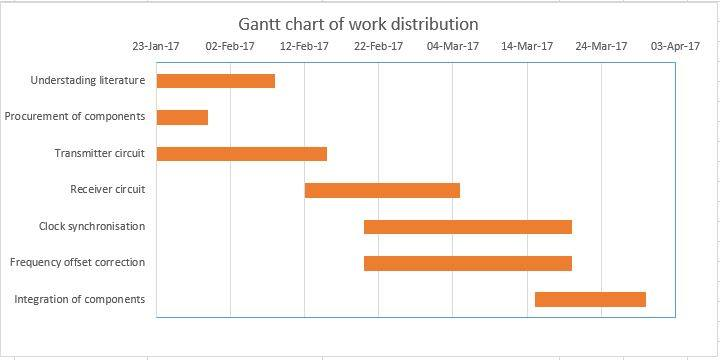
\includegraphics[scale=0.5]{Gantt_chart}
% \section{Project Implementation}
% % At this stage, you need to submit a BOM (Bill of Materials). Apart from the components decide your testing strategy - how to test, needed tools, precautions and feasibility Assessment (resources, risks).  What is the deliverable of the work and demo possible in reality?
% Components Required:
% \begin{itemize}
% \item Led (white) : Rs 50
% \item Bias Tee Inductor and Capacitor
% \item Photodiode (detector) : Rs 50
% \item OP-Amp (for driver circuit) [TL082/ UA741] : Rs 20
% \item PLL IC (CD4046B)
% \item DSP Board 
% \item Microcontroller (Tiva C LaunchPad) : Rs 1800
% \end{itemize}

% The testing strategy would be mainly around on sending different bit patterns and seeing and noting the error in each of them. The final aim is to transfer a file using the communication link. We would go about to reach this final aim in small steps of sending different bit patterns of varying length and estimate and establish the fidelity of the link. There is no specific requisites for the same except for the something that can collect and tally the data sent and received which would be done using our laptops. There aren’t any specific risks associated with this and does not demand any specific setup as such. In fact that is the challenge of not having a very specific arrangement to use the communication link. 
% \section{Deliverables}
% % Spell out the project deliverables - what you would demonstrate during the evaluations
% % (It is expected that for the first evaluation (1st week of Feb) roughly 30% of work is ready. You will have to demonstrate the subsystems that are ready. For the second evaluation (2nd week of March) 60 to 80% of your work should be over and you should be working on your final PCB, box etc. We expect a draft version of your final report submitted by the 1st week of April. For the final evaluation (April 10-14) you need to give a brief presentation (20 min) and a demo of your project.)

% \begin{itemize}
% \item By first week of February, we hope to get done with
%   \begin{itemize}
%   \item Understanding Literature
%   \item Procurement of Components
%   \item Finishing the Transmitter Circuit
%   \item Getting Started with the Receiver 
%   \end{itemize}

% \item By second week of March, we hope to accomplish

%   \begin{itemize}
%   \item Finish Tackling the Problem of Clock Synchronization and Frequency offset
%   \item Start integrating the components.
%   \end{itemize}

% \item By first week of April, we hope to accomplish
%   \begin{itemize}
%   \item After second evaluation, we get started with testing of the circuit. We will start off with 10 kbps, correct the errors which come in the way and in the end   hope to get the desired speed of 1Mbps. 
%   \end{itemize}
% \end{itemize}


\end{document}

